%!TEX program=lualatex

\def\LectureName/{General Physics I}
%\def\LectureNumber/{}
%\def\LectureDate/{}
\PassOptionsToPackage{fleqn}{amsmath}
\PassOptionsToPackage{hyperfootnotes=false}{hyperref}
\documentclass[11pt,pdfa,lastpage]{MishoNote}
\title{General Physics I: Vector Boot Camp}
\author{Sho Iwamoto}
\hypersetup{
  pdflang={en-US},
  pdfauthortitle={Assistant Professor, National Sun Yat-sen University},
  pdfsubject={Vector Boot Camp (Basic) as a preparation to General Physics 1 lecture.},
  pdfcontactemail={iwamoto@g-mail.nsysu.edu.tw},
  pdfcontacturl={https://www2.nsysu.edu.tw/iwamoto/},
  pdfcaptionwriter={Sho Iwamoto},
  pdfcopyright={2024 Sho Iwamoto\textLF This document is licensed under the Creative Commons CC BY–NC 4.0 International Public License.},
  pdflicenseurl={https://creativecommons.org/licenses/by-nc/4.0/},
}

\usepackage{GP}
\usepackage{pgfornament}
\setlist{itemsep=4pt}
\def\thesection{B}

\newcommand\hrefFN[2]{\href{#1}{#2}\addnote{\url{#1}}}
\newcommand\starskip{\bigskip\begin{center}\pgfornament[width=7cm]{88}\end{center}\medskip}
\newcommand\fakebullet{\makebox[2.5em][r]{\textbullet\kern.5em}}
\makeatletter
\RenewDocumentCommand\new@problem{mm}{%
  \stepcounter{Problem}\item[\kern-2em\kern-\labelsep{\makebox[4.5em][r]{%
        \IfValueTF{#2}{\csname G#2\endcsname}{}{\sffamily\bfseries[\Alph{Problem}]}}}]\relax}
\makeatother

\let\origfootnote\footnote
\let\origfootnoterule\footnoterule

\begin{document}%
\title{Vector Boot Camp}
\begin{maketitle}
\let\footnote\origfootnote
\let\footnoterule\origfootnoterule

\subsection*{Preface}
Vectors are a familiar concept from high school mathematics, and you likely already have a good understanding of them.
However, vectors are far more important than you might realize.
They are arguably one of the most crucial mathematical concepts not only in science but also in the modern society.
.
A vector can take on many forms: in high school math, it's often seen as two or three numbers; in university physics, it's represented as an arrow; and in university mathematics, it's an element of a vector space.
What you have learned is just the beginning, and you will need to develop a deeper and more versatile understanding of vectors.

This Boot Camp is designed to bridge the gap between high school math and university physics.
You will be well-prepared to tackle the challenges and opportunities of advanced physics studies.
Good luck!

\subsection*{Remarks}
This Boot Camp contains all the topics that you will need in General Physics 1 and 2 lectures.
Most of the topics will be discussed during Sho's lecture, so you do not have to do all by yourself. Still, it is beneficial if you can learn these topics by yourselves, so that you can focus more on physics during the lectures.

\medskip

Sho never provides you with solutions\addnote{Think why. Sho thinks that proding solutions is against the integrity (or a moral) as a scientist.} \Emph{You students} need to make the solution. To this end,
\begin{miniitemize}
  \item Share your answers to other colleagues, using LINE or \hrefFN{https://docs.google.com/}{Google Docs}. Compare your answers with theirs.
  \item Ask questions to colleagues, to the TA, or to Sho. You can utilize Sho's \hrefFN{https://www2.nsysu.edu.tw/iwamoto/}{office hours}.
\end{miniitemize}

\OutputNote

\enlargethispage{-5em}

\makeatletter
\begin{tikzpicture}[remember picture,overlay]
  \begingroup
  \fontsize{9}{13}\selectfont
    \node[xshift=\@total@leftsep,yshift=25.5mm,anchor=south west,align=left,text width=\textwidth] at (current page.south west) {%
      \href{https://creativecommons.org/licenses/by-nc/4.0/}{
\includegraphics[width=2.2cm]{../figs/by-nc.pdf}}\\[.4em]
      \noindent\textsf{\color{gray}%
      Visit \url{https://github.com/misho104/LecturePublic} for further information, updates, and to report issues.}\par
    };
    \node[xshift=-\@total@leftsep+26mm,yshift=32mm,align=left,text width=\textwidth,anchor=south east] at (current page.south east) {%
      \noindent\textsf{\color{gray}%
      This document is licensed under
      \href{https://creativecommons.org/licenses/by-nc/4.0/}{the Creative Commons CC--BY--NC 4.0 International Public License.}\\
      You may use this document only if you do in compliance with the license.}\par
    };
  \endgroup
\end{tikzpicture}
\makeatother

\end{maketitle}
\newpage


\newsavebox{\VectorSetA}
 \begin{lrbox}{\VectorSetA}
 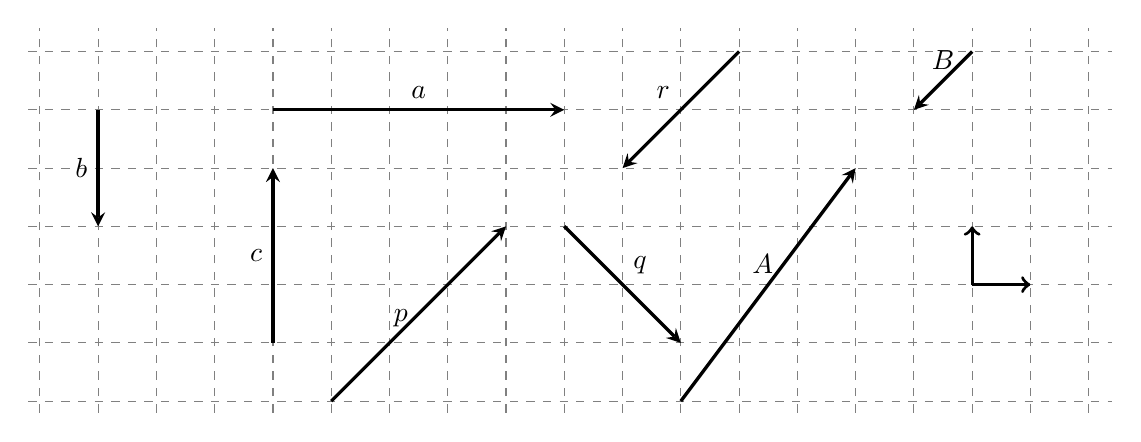
\begin{tikzpicture}[scale=0.74]
  \draw[help lines,thin,dashed] (-3.2,-1.2) grid ++(18.6,6.6);
  %\draw[->]                     (-3.2,  0 ) --   ++(18.6, 0 ) node[below left,xshift=1.3mm]{$x$};
  %\draw[->]                     (  0 ,-1.2) --   ++( 0  ,6.6) node[below left,yshift=1.3mm]{$y$};
  %\coordinate (O) at (0,0) node [below left,xshift=.5mm,yshift=.5mm] at (O) {O}; %\fill (O) circle (4pt);
  \draw[-stealth, very thick] (1,4)--node [above]{$\vc a$} ++(5,0);
  \draw[-stealth, very thick] (-2,4)--node [left]{$\vc b$} ++(0,-2);
  \draw[-stealth, very thick] (1, 0)--node [left]{$\vc c$} ++(0,3);
  \draw[-stealth, very thick] (2,-1)--node [above left,yshift=-3mm]{$\vc p$} ++(3,3);
  \draw[-stealth, very thick] (6,2)--node [above right]{$\vc q$} ++(2,-2);
  \draw[-stealth, very thick] (9,5)--node [above left]{$\vc r$} ++(-2,-2);
  \draw[-stealth, very thick] (8,-1)--node [above left,xshift=2mm]{$\vc A$} ++(3,4);
  \draw[-stealth, very thick] (13,5)--node [above]{$\vc B$} ++(-1,-1);
  \draw[->,very thick] (13,1)--node [below]{$\vvex$} ++(1,0);
  \draw[->,very thick] (13,1)--node [left] {$\vvey$} ++(0,1);
  %\fill (O) circle (4pt) (A) circle (4pt) (B) circle (4pt) (C) circle (4pt) (D) circle (4pt);
  \end{tikzpicture}
\end{lrbox}
\newsavebox{\VectorSetB}
 \begin{lrbox}{\VectorSetB}
 \begin{tikzpicture}[scale=0.74]
  %\draw (0,0) rectangle ++ (7,4);
  \coordinate (A) at (1,3) node [above,xshift=-2mm] at (A) {A};
  \coordinate (B) at (5,5) node [right,yshift=2mm] at (B) {B};
  \coordinate (C) at (6,0) node [above,xshift=2mm] at (C) {C};
  \fill (A) circle (4pt) (B) circle (4pt) (C) circle (4pt);
  \end{tikzpicture}
\end{lrbox}
\newsavebox{\VectorSetC}
\begin{lrbox}{\VectorSetC}
  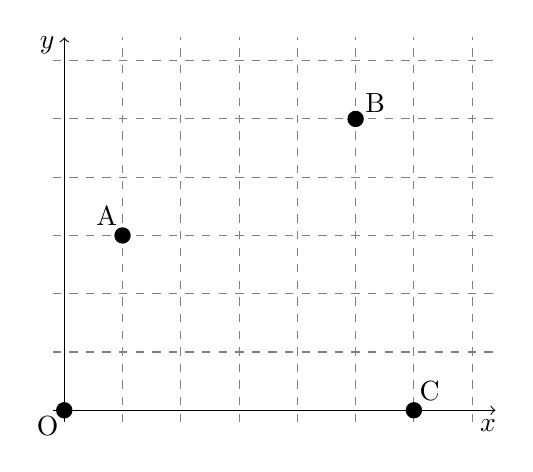
\begin{tikzpicture}[scale=0.74]
   \draw[help lines,thin,dashed] (-0.2,-0.2) grid ++(7.6,6.6);
   \draw[->]                     (-0.2,  0 ) --   ++(7.6, 0 ) node[below left,xshift=1.3mm]{$x$};
   \draw[->]                     (  0 ,-0.2) --   ++( 0  ,6.6) node[below left,yshift=1.3mm]{$y$};
   \coordinate (O) at (0,0) node [below left,xshift=.5mm,yshift=.5mm] at (O) {O}; \fill (O) circle (4pt);
  \coordinate (A) at (1,3) node [above,xshift=-2mm] at (A) {A};
  \coordinate (B) at (5,5) node [right,yshift=2mm] at (B) {B};
  \coordinate (C) at (6,0) node [above,xshift=2mm] at (C) {C};
  \fill (A) circle (4pt) (B) circle (4pt) (C) circle (4pt);
  \end{tikzpicture}
\end{lrbox}
\subsection{Definition of Vectors}
\begin{definition}{Vectors (for physics)}{def:vec}
\begin{miniitemize}
  \item A vector is a physical quantity that has both \Emph*{magnitude} and \Emph*{direction}.
  \item We describe them by $\vc a$, $\vc A$, $\vc p\w F$, etc.\addnote{%
    Professionals use boldface, e.g., $\mathbf{a}$, $\mathbf{A}$, $\mathbf{p}\w F$, etc., but in this lecture we only use the beginners' style.},
    and their magnitudes by $|\vc a|$, $|\vc A|$, $|\vc p\w F|$, etc.
  \item We often describe them by arrows. The arrows' direction should match the vector's direction. The arrows' length should be \emph{proportional to} the vector's magnitude.
\end{miniitemize}
\end{definition}
\OutputNote

\begin{definition}{Vector quantity and Scalar quantity}{def:vecsca}
  \begin{miniitemize}
    \item Physical quantities with direction are called \Emph*{vector quantity}.
    \begin{miniitemize} \item They can be described by vectors.\addnote{%
      If the space considered is one-dimensional, we can describe the direction by $+$ or $-$ and a vector quantity can be described by a number. Here, however, \Emph{you} must specify which direction is positive.} \end{miniitemize}
    \item Physical quantities without direction are called \Emph*{scalar quantity}.
    \begin{miniitemize} \item They can be described by numbers.\end{miniitemize}
    \item Consider a vector quantity $\vc A$. Its magnitude $|\vc A|$ is a scalar quantity.
  \end{miniitemize}
  \end{definition}
\OutputNote
For example, \Emph*{mass} $m$ and \Emph*{temperature} $T$ are scalar quantities. \Emph*{Velocity} $\vc v$ is a vector quantity and its magnitude $|\vc v|$ (it has a special name ``\Emph*{speed}'')  is a scalar quantity. Acceleration $\vc a$ is a vector quantity.

\begin{quizzes}
  \Quiz[S] Choose vector quantities. Choose scalar quantities.
  \begin{menumerate}[labelsep=0em,labelwidth=0em,itemindent=1em,label={},leftmargin=0.3em]{4}
    \item temperature
    \item air pressure
    \item wind speed
    \item velocity
    \item electric charge
    \item Sho's height
    \item Sho's weight
    \item Sho's mass
    \item city name
    \item position
    \item time difference
    \item time
    \item duration
    \item distance
    \item kilometer
    \item resistor
    \item resistance
    \item conductor
    \item conductance
    \item conductivity
  \end{menumerate}
\end{quizzes}

\newpage
\subsection{How to describe directions}
\Remark{
  Using natural English is nice, but it is more important, and thus we should pay greater attention, to ensure that the expression is clear and does not cause any misunderstanding.
}
\paragraph{Basic}
\emph{We} need to learn how to describe directions of vectors \Emph{in English}. The easiest one is
\begin{tabbing}
 \fakebullet \= downward   \== toward the bottom      \=\kill
 \fakebullet \> leftward   \>= toward the left        \>= to the left\\[\itemsep]
 \fakebullet \> rightward  \>= toward the right       \>= to the right\\[\itemsep]
 \fakebullet \> upward     \>= toward the top         \>= to the top\\[\itemsep]
 \fakebullet \> downward   \>= toward the bottom      \>= to the bottom
% \item forward / backward (if the front and back are obvious, e.g., a car or bicycle)
\end{tabbing}
If you need to describe the third dimension which is perpendicular to the textbook's page or the sheet (or the blackboard), you can use
\begin{tabbing}
  \fakebullet \= out of the \= (sheet | page | blackboard) \= = away from the \= (sheet | page | blackboard)\kill
  \fakebullet \> into   the \> (sheet | page | blackboard) \> = toward    the \> (sheet | page | blackboard)\\[\itemsep]
  \fakebullet \> out of the \> (sheet | page | blackboard) \> = away from the \> (sheet | page | blackboard)
\end{tabbing}
For 2d case, \Emph{once you specify the ``north'' direction,} you can use the following expressions:
\begin{miniitemize}
 \item northward, southward, eastward, westward (= (to | toward) the north, etc.)
 \item northwestward, southwestward, etc. (= (to | toward) the northwest, etc.)
\end{miniitemize}

\paragraph{With axes}
Usually, we define $x$-axis and $y$-axis (and $z$-axis, if 3d). \Emph{If such axes are defined} (or once you have defined them), we can use
\begin{tabbing}
  \fakebullet \= in the negative $x$-direction \= = in the $-x$ direction\kill
  \fakebullet \> in the positive $x$-direction \> = in the $+x$ direction\\[\itemsep]
  \fakebullet \> in the positive $y$-direction \> = in the $+y$ direction\\[\itemsep]
  \fakebullet \> in the negative $x$-direction \> = in the $-x$ direction\\[\itemsep]
  \fakebullet \> in the negative $y$-direction \> = in the $-y$ direction
 \end{tabbing}
In particular, for 2d cases, we can use the angle from the positive $x$-axis (counterclockwise):
 \begin{miniitemize}
  \item $30^\circ$ from the $+x$ axis (= $30^\circ$ counterclockwise from the positive $x$-axis)
  \item $90^\circ$ from the $+x$ axis (= in the $+y$ direction)
  \item $170^\circ$ from the $+x$ axis (= $10^\circ$ clockwise from the negative $x$-axis)
  \item $-15^\circ$ from the $+x$ axis (= $15^\circ$ clockwise from the positive $x$-axis)
  \item angle $\theta$ from the $+x$ axis, where $\tan\theta=0.1$ and $0<\theta<\pi/2$.
 \end{miniitemize}
Sometimes the word ``the horizontal'' is useful:
\begin{miniitemize}
  \item $10^\circ$ above the horizontal / $30^\circ$ below the horizontal
\end{miniitemize}
\Remark{It is difficult to describe general 3d directions by words. For this purpose, we usually use mathematical expressions (i.e., vectors).}

\paragraph{Rotations}
To describe the direction of rotation, we use
\begin{miniitemize}
  \item clockwise / counterclockwise
\end{miniitemize}
If you have an arrow and discuss rotations about the arrow, you can use the following expressions:
\begin{miniitemize}
  \item following the right-hand rule (= counterclockwise when viewed from the arrow's direction)
  \item following the left-hand rule (= clockwise when viewed from the arrow's direction)
\end{miniitemize}
We will often use these expressions in General Physics 2.

\newpage

\subsection{Vectors: Magnitude and Direction}
In this Boot Camp, we forget about physics\addnote{%
 We forget units and significant figures, which you will learn in the beginning of General~Physics~1 lectures. In other words, in the lectures, \Emph{you must not forget units and significant figures} of vector quantities.
}.
Focusing on mathematics, we will discuss vectors in its mathematical aspects.
We will begin with a few more expressions useful for vectors.

If the angle between $\vc a$ and $\vc b$ is $90^\circ$, we say
\begin{tabbing}
  \fakebullet \= \kern16em \=\kill
  \fakebullet \> $\vc a$ is \Emph{perpendicular to} $\vc b$. \> \fakebullet $\vc a$ and $\vc b$ are perpendicular to each other.\\[\itemsep]
  \fakebullet \> $\vc a$ is orthogonal to $\vc b$.   \>    \fakebullet $\vc a$ and $\vc b$ are orthogonal  to each other.\\[\itemsep]
  \fakebullet \> $\vc a$ is normal to $\vc b$.       \>    \fakebullet $\vc a$ and $\vc b$ are normal to each other.
 \end{tabbing}
(all of them are correct but the first one is the most common). If the angle is $0^\circ$, we say\addnote{%
\Emph{Avoid} the word ``parallel'' because some people think it includes both $0^\circ$ and $180^\circ$ cases. Clarity is important in science.}
\begin{tabbing}
  \fakebullet \= \kern16em \=\kill
  \fakebullet \> $\vc a$ is \Emph{in the same direction as} $\vc b$. \> \fakebullet $\vc a$ and $\vc b$ are in the same direction.
\end{tabbing}
Finally, if the angle is $180^\circ$,
\begin{tabbing}
  \fakebullet \= \kern16em \=\kill
  \fakebullet \> $\vc a$ is \Emph{anti-parallel to} $\vc b$. \> \fakebullet $\vc a$ and $\vc b$ are anti-parallel.\\[\itemsep]
  \fakebullet \> $\vc a$ is opposite to $\vc b$.      \> \fakebullet $\vc a$ and $\vc b$ are in opposite directions.
\end{tabbing}

\OutputNote



\begin{problems}
 \Problem[S] Vectors are drawn on the grid, which has a spacing of 1. Answer the following questions.
 \par\smallskip\par\usebox{\VectorSetA}

\begin{enumerate}
  \item Describe the direction (in English words) and magnitude of each vector. Try to use multiple expressions.
  \item Describe relationship between the directions of the following vector pairs:\\
   ($\vc a$ and $\vc b$), ($\vc b$ and $\vc c$), ($\vc p$ and $\vc q$), ($\vc p$ and $\vc r$), ($\vvex$ and $\vvey$), and ($\vc a$ and $\vvex$).\\
   For example, ``$\vc a$ is perpendicular to $\vc b$''.
\end{enumerate}

\end{problems}

\newpage


\subsection{Vector Basics}
These are a few basic things that you have learned in highschool:
\begin{itemize}
\item \Emph*{(Zero vector)} There is a special vector $\vc 0$. Its length is $0$ (zero) and it has no direction.
\item \Emph*{(Scalar multiplication)} If $\vc v$ is a vector, $2\vc v$ and $-3\vc v$ are both vectors.
\item \Emph*{(Addition)} If $\vc p$ and $\vc q$ are vectors, $\vc p + \vc q$ is a vector.
\end{itemize}
By extending the last two items, we can obtain the following statement.
\begin{itemize}
  \item \Emph*{(Linear combination)} If $a$ and $b$ are scalars (i.e., real numbers) and $\vc p$ and $\vc q$ are vectors,
  \[ a\vc p+b\vc q \]
  is a vector. Here, $a$ and $b$ can be positive, zero, or negative.
\end{itemize}

\begin{problems}
 \Problem[S] Vectors are drawn on the grid, which has a spacing of 1.
 \par\smallskip\par\usebox{\VectorSetA}
 \begin{enumerate}
   \item Describe $\vc a$ by using $\vvex$ (and a number).  Describe $\vc b$ and $\vc c$ by using $\vvey$.
   \item Describe $\vc B$ by using $\vc r$. Describe $\vc p$ by using $\vc r$.
   \item Describe $\vc A$ and $\vc B$ by using $\vvex$ and $\vvey$.
   \item Describe $\vvex$ and $\vvey$ by using $\vc A$ and $\vc B$.\\
    \Hint{See your answer of the previous problem.}
   \item Draw a vector $\vc \beta$ that is in the same direction as $\vc b$ and $|\vc \beta|=1$.
 \end{enumerate}
 \Problem[S] Consider a vector $\vc s$ whose length is 3, i.e., $|\vc s|=3$.
 \begin{enumerate}
   \item Calculate the magnitude of $2\vc s$, $-3\vc s$, and $0\vc s$.
   \item Calculate the magnitude of $\dfrac{\vc s}{|\vc s|}$.
   \item Describe relationship between the directions of the following vector pairs:\\
        ($\vc s$ and $4\vc s$), ($0.1\vc s$ and $-4\vc s$), and ($\vc s$ and $\dfrac{\vc s}{|\vc s|}$).
   \item Let $\vc S=-3\vc s$ and $k$ be a real number. Find the direction and magnitude of $\vc s+k\vc S$.
 \end{enumerate}
\end{problems}
\newpage

Here is one more important concept:
\begin{itemize}
  \item \Emph*{(Unit vector)} If a vector has a magnitude of one, it is called a \Emph*{unit vector}.
\end{itemize}
If $\vc a$ is not the zero vector,
\begin{itemize}
  \item the unit vector in the same direction as $\vc a$ is given by $\dfrac{\vc a}{|\vc a|}$; it is denoted by $\vc{\hat{a}}$ (hat + arrow);
  \item the unit vector that is anti-parallel to $\vc a$ is given by $-\dfrac{\vc a}{|\vc a|}$\quad($=-\vc{\hat{a}}$).
\end{itemize}
\Remark{In the textbook, vectors are written by $\vc{\mathbfup{a}}$ and unit vectors are by $\hat{\mathbfup{a}}$. (Some of you will be confused by this notation in General Physics 2.)
Although the notation is a bit messy, Sho will always use $\vc a$ and $\vc{\hat a}$.}



\begin{problems}
 \Problem[A] Consider $\vc s$ and $\vc t$, which satisfy $|\vc s|=3$ and $|\vc t|=2$. Here, $k>0$.
 \begin{enumerate}
   \item Find the unit vector whose direction is the same as $\vc s$.
   \item Find the unit vector whose direction is the same as $-2\vc t$.
   \item Find the unit vector whose direction is the same as $4\vc s+3\vc t$.
   \item Find the unit vector anti-parallel to $\vc s$.
   \item Find the vector which is anti-parallel to $\vc s$ and has a magnitude of 12.
   \item Find the vector which is in the same direction as $\vc t$ and has a magnitude of $k$.
 \end{enumerate}
\end{problems}

You will see unit vectors many times in the following exercises.

\newpage
\subsection{Inner product}
We use this definition, which may be different from what you learned in highschool.
\begin{definition}{Inner product}{def:inner}
  For vectors $\vc a$ and $\vc b$, the \Emph*{inner product} of $\vc a$ and $\vc b$ is defined by
  \[ \vc a\cdot\vc b\deq|\vc a||\vc b|\cos\theta, \qquad \text{where $\theta$ is the angle between $\vc a$ and $\vc b$.} \]
\end{definition}
\begin{problems}
  \Problem[A] Prove the following equations \Emph{from the above definition}.
  \begin{enumerate}
    \item $\vc a\cdot\vc b=\vc b\cdot\vc a$ for any vectors $\vc a$ and $\vc b$.
    \item $(k\vc a)\cdot\vc b=k(\vc a\cdot\vc b)$ for any vectors $\vc a$ and $\vc b$ and any number $k$.
    \item $\vc a\cdot\vc a=|\vc a|^2$ for any vector $\vc a$.
    \item $\vc a\cdot\vc b=0$ if $\vc a=\vc 0$, $\vc b=\vc 0$, or $\vc a$ is perpendicular to $\vc b$.
    \item $-|\vc a||\vc b|\le \vc a\cdot\vc b\le|\vc a||\vc b|$ for any vectors $\vc a$ and $\vc b$.
  \end{enumerate}
\end{problems}
We can also prove $(\vc a+\vc b)\cdot\vc c=\vc a\cdot\vc c+\vc b\cdot \vc c$ from the above definition. However, the proof is a bit technical and thus skipped. You will anyway use this equation.

\medskip

\noindent\Emph{The next two problems are the most important ones in this Boot Camp.}
\begin{problems}
  \Problem[S] Two vectors $\vc x$ and $\vc y$ satisfy $|\vc x|=|\vc y|=1$ and $\vc x\cdot\vc y=1/2$. 
  \begin{enumerate}
    \item Calculate the angle between $\vc x$ and $\vc y$.
    \item Expand $|a\vc x+b\vc y|^2$ and calculate its value. Calculate $|a\vc x+b\vc y|$.
  \end{enumerate}
  Now, assume $\vc s=3\vc x+3\vc y$ and $\vc t=2\vc x-\vc y$. Also, let $\vc{\hat s}$ be the unit vector whose direction is the same as $\vc s$.
  \begin{enumerate}[resume]
    \item Calculate $|\vc s|$, $|\vc t|$, and $\vc s\cdot\vc t$. Find the angle between $\vc s$ and $\vc t$.
    \item Describe $\vc{\hat s}$. \Hint{The answer will contain $\vc x$ and $\vc y$.}
    \item Assume $\vc u=\vc x+k\vc y$ is perpendicular to $\vc s$. Find the value of $k$.
  \end{enumerate}
  \Problem[S] Two vectors $\vvex$ and $\vvey$ satisfy $|\vvex|=|\vvey|=1$ and $\vvex\cdot\vvey=0$. 
  \begin{enumerate}
    \item Calculate the angle between $\vvex$ and $\vvey$.
    \item Expand $|a\vvex+b\vvey|^2$ and calculate its value. Calculate $|a\vvex+b\vvey|$.
  \end{enumerate}
  Now, assume $\vc p=a\vvex+b\vvey$, which is not $\vc 0$, and $\vc q=3\vvex+4\vvey$.
  \begin{enumerate}[resume]
    \item Calculate $|\vc p|$, $\vc p\cdot\vvex$, and $\vc p\cdot\vvey$. Check that $\vc p=(\vc p\cdot\vvex)\vvex+(\vc p\cdot\vvey)\vvey$.
    \item Calculate $|\vc q|$, $\vc q\cdot\vvex$, $\vc q\cdot\vvey$, and $\vc p\cdot\vc q$.
    \item Find the unit vector whose direction is the same as $\vc p$.
  \end{enumerate}
\end{problems}
\begin{problems}
  \Problem[S] Let $ \vc a=a_1\vc i+a_2\vc j+a_3\vc k$ and $\vc b=b_1\vc i+b_2\vc j+b_3\vc k$,
  where $\vc i$, $\vc j$, and $\vc k$ are (any) vectors.
  \begin{enumerate}
    \item Expand $|\vc a|^2$ and $\vc a\cdot\vc b$.
  \end{enumerate}
  Now, assume they satisfy $|\vc i|=|\vc j|=|\vc k|=1$ and $\vc i\cdot\vc j=\vc j\cdot\vc k=\vc k\cdot\vc i=0$.
  \begin{enumerate}[resume]
    \item Simplify the answer of the previous question.
    \item Calculate the angle between $\vc a$ and $\vc b $.
    \item Write down $\vc{\hat a}$ (the unit vector in $\vc a$'s direction) by using $a_{1,2,3}$, $\vc i$, $\vc j$, and $\vc k$.
  \end{enumerate}
\end{problems}


\begin{problems}
  \Problem[A] Three vectors $\vc A$, $\vc B$, and $\vc C$ satisfy $|\vc A|=2$, $|\vc B|=3$, $\vc A\cdot \vc B=3\sqrt2$, and $\vc A\cdot\vc C=-1$.
  \begin{enumerate}
    \item Find the angle between $\vc A$ and $\vc B$.
    \item Calculate $|\vc A+\vc B|^2$, $|\vc A-\vc B|^2$, and $|2\vc A+4\vc B|^2$.
    \item Calculate $(\vc A-2\vc B)\cdot(2\vc A+\vc B+\vc C)+2\vc B\cdot\vc C$.
    \item Assume $|\vc A+k\vc B|=\sqrt{10}$. Find the value of $k$.
    \item Assume $\vc B+c\vc C$ is perpendicular to $\vc A$. Find the value of $c$.
    \item What do we know about the values of $|\vc C|$ and $|\vc A-\vc C|$?
  \end{enumerate}
  \Problem[C] Two vectors $\vvex$ and $\vvey$ satisfy  $|\vvex|=|\vvey|=1$ and $\vvex\cdot\vvey=0$.
Define
\begin{align*}
  \vc{a_x}&=\frac12\vvex+\frac12\vvey,&
  \vc{f_x}&=\vvex\cos\theta+\vvey\sin\theta,  \\
  \vc{a_y}&=\vvex+\frac12\vvey,&
  \vc{f_y}&=-\vvex\sin\theta+\vvey\cos\theta.
\end{align*}
First, consider $\vc A=A\vc{a_x}+B\vc{a_y}$.
\begin{enumerate}
  \item Calculate $\vc{a_x}\cdot\vc{a_y}$, $|\vc{a_x}|$, and $|\vc {a_y}|$.
  \item Calculate $|\vc A|$.
  \item Write down $\vc A$ by using $\vc{e_x}$, $\vc{e_y}$, $A$, and $B$.
\end{enumerate}
Next, consider $\vc P=P\vc{f_x}+Q\vc{f_y}$ and $\vc S=S\vc{f_x}+T\vc{f_y}$.
\begin{enumerate}[resume]
  \item Calculate $\vc{f_x}\cdot\vc{f_y}$, $|\vc{f_x}|$, and $|\vc {f_y}|$.
  \item Calculate $\vc P\cdot\vc S$, $|\vc P|$, and $|\vc S|$.
  \item Write down $\vc P$ by using $\vvex$, $\vvey$, $P$, $Q$, and $\theta$.
  \item Write down $\vvex$ and $\vvey$ by using $\vc{f_x}$, $\vc{f_y}$, and $\theta$.
  \item Check the following equation:
  \[ \vc P=(\vc P\cdot\vc{f_x})\vc{f_x}+(\vc P\cdot\vc{f_y})\vc{f_y}
  =(\vc P\cdot\vc{e_x})\vc{e_x}+(\vc P\cdot\vc{e_y})\vc{e_y}\]
\end{enumerate}
\end{problems}
\newpage
\subsection{Cross product}\label{sec:cross}
The definition of the cross product may also be different from highschool mathematics.
\begin{definition}{Cross product}{def:cross}
  For vectors $\vc a$ and $\vc b$, the \Emph*{cross product} of $\vc a$ and $\vc b$ is defined as follows:
\begin{itemize}
  \item it is a vector and denoted by $\vc a\times\vc b$;
  \item its magnitude $|\vc a\times\vc b|$ is given by $|\vc a||\vc b|\sin\theta$, where $\theta$ is the angle between $\vc a$ and $\vc b$;
  \item if $|\vc a\times\vc b|\neq 0$, its direction is specified so that
  \begin{itemize}
    \item $\vc a\times\vc b$ is perpendicular to both $\vc a$ and $\vc b$;
    \item The triplet $(\vc a,\vc b,\vc a\times\vc b)$ satisfies the right-hand rule.
  \end{itemize}
\end{itemize}
\end{definition}
Here, ``$(\vc p,\vc q,\vc r) $ satisfies the right-hand rule'' means that if you hold your right hand so that your thumb points in the direction of $\vc p$ and your index finger $\vc q$, then your middle finger points in the direction of $\vc r$. Or, if you draw $\vc p$ upward and $\vc q$ leftward on a sheet, then $\vc p\times\vc q$ points out of the sheet toward you.%
\mbox{$^{\text{\ref{Note:vec}}}$}\
\NoteBox[label=Note:vec]
 More precisely, if $\vc p$ and $\vc q$ are on the sheet and the direction of $\vc q$ is $\theta$ clockwise from $\vc p$ with $0^\circ<\theta<180^\circ$, then $\vc p\times\vc q$ is normal to the sheet and points out of the sheet. If $180^\circ<\theta<360^\circ$, then $\vc p\times \vc q$ is normal to the sheet and points toward the sheet.
\endNoteBox
\begin{problems}
  \Problem[A] Prove the following equations \Emph{from the above definition}.
  \begin{enumerate}
    \item $\vc a\times\vc a=\vc 0$.
    \item $\vc a\times\vc 0=\vc 0\times\vc a=\vc 0$.
    \item $\vc a\times\vc b=\vc 0$ if $\vc a$ and $\vc b$ are parallel or anti-parallel.
    \item $\vc a\times\vc b=-\vc b\times\vc a$.
    \item $(k\vc a)\times\vc b=\vc a\times(k\vc b)=k(\vc a\times\vc b)$.
    \item $0\le|\vc a\times\vc b|\le|\vc a||\vc b|$.
    \item $\vc a\cdot(\vc a\times\vc b)=0$.
    \item $(\vc a\cdot\vc b)^2+|\vc a\times\vc b|^2=|\vc a|^2|\vc b|^2$.
  \end{enumerate}
\end{problems}
We can also prove $(\vc a+\vc b)\times\vc c=\vc a\times\vc c+\vc b\times \vc c$ from the above definition. However, the proof is extremely technical and thus skipped. You need this equation in the next problem.
\begin{problems}
  \Problem[S] Three vectors $\vvex$, $\vvey$, and $\vvez$ satisfy
  \[ |\vvex|=|\vvey|=|\vvez|=1,
   \quad \vvex\times\vvey=\vvez,
   \quad \vvey\times\vvez=\vvex,
   \quad \vvez\times\vvex=\vvey.
  \]
  \begin{enumerate}
    \item Calculate $\vvex\cdot\vvey$. Find the angles among $\vvex$, $\vvey$, and $\vvez$.
    \item Expand $(a\vvex+b\vvey+c\vvez)\times(p\vvex+q\vvey+r\vvez)$ and simplify.
  \end{enumerate}
\end{problems}


\newpage
\subsection[Operation on Vectors]{Operation on vectors — Introduction to the Vector/Scalar/Not game}
We have seen all the operations. Namely, (only) the following operations are possible on vectors:
\begin{tabbing}
\fakebullet \= \Emph*{scalar multiplication}:~~\= $\vc a\times\vc b$\quad \= \kill
\fakebullet \> \Emph*{magnitude}:              \> $|\vc a|$           \> ($\leftarrow$ scalar)\\
\fakebullet \> \Emph*{scalar multiplication}:~~\> $k\vc a$            \> ($\leftarrow$ vector)\\
\fakebullet \> \Emph*{addition}:               \> $\vc a+\vc b$       \> ($\leftarrow$ vector)\\
\fakebullet \> \Emph*{inner product}:          \> $\vc a\cdot\vc b$   \> ($\leftarrow$ scalar)\\
\fakebullet \> \Emph*{cross product}:          \> $\vc a\times\vc b$  \> ($\leftarrow$ vector)
\end{tabbing}
where $k$ is a scalar and $\vc a$ and $\vc b$ are vectors. Any complicated symbols, such as
\[
\frac{\vc a\times \vc b+(\vc x\cdot\vc y)\vc d}{(\vc a\cdot\vc b)|\vc b\times\vc c+\vc d|}
\]
can be obtained by combining these five operations.
\Remark{The numerator is the sum of two vectors: the first one is $\vc a\times\vc b$, and the second one is $\vc d$ multiplied by a scalar (number) $\vc x\cdot\vc y$. The denominator is made of two numbers; the first number is $\vc a\cdot\vc b$, while in the second, $\vc b\times\vc c$ is a vector, so it can be added to $\vc d$, and then its magnitude is evaluated.}

In other words, \Emph{we cannot apply any other operations} except for these five. Namely,
{
\color{AltDefA}
\begin{align*}
   (\vc a)^2,
 && \frac{1}{\,\vc a\,},
 && k+\vc a,
 && \vc a\vc b,
 && \sqrt{\vc a},
 && \frac{\vc a}{\,\vc a\,},
 && a+\vc a,
 && \vc a\cdot\vc b+\vc a\times\vc b,
 && (\vc a+\vc b)\vc c
\end{align*}
}
are all invalid expression; they do not express any mathematical concept.

Now, you need to distinguish \Emph{which is vector, which is scalar, and which is invalid}.
\begin{problems}
\Problem[S] For each expression, answer \Emph*{V} if it is vector; \Emph*{S} if it is scalar, and \Emph*{N} if it is an invalid expression (neither vector nor scalar).\\
\Hint[]{Notice that symbols with an arrow are vectors and symbols without an arrow are scalars.}
\begin{align*}\def\baselinestretch{2}
  & 3+|\vc a|
  && \vc a-\vc b
  && \vc a\vc b
  && \vc a/\vc b
  && \vc p\times(\vc q\times\vc r)
\\[.5em]& 3\vc a
  && \vc 0+1
  && \vc 0
  && -\vc a
  && \vc p\cdot(\vc q\times\vc r)
\\[.5em]& 3\times\vc a
  && \vc k\times\vc a
  && x+|\vc a|
  && |\vc a|^{-1}\vc a
  && p\times(\vc q\times\vc r)
\\[.5em]& \frac{1}{\vc x+\vc y}
  && \frac{x+y}{|\vc x+\vc y|}
  && \frac{\vc x+\vc y}{|\vc x+\vc y|}
  && \frac{\vc x+\vc y}{\vc x+\vc y}
  && \vc p(\vc q\times\vc r)
\\[.5em]& \frac{1}{(\vc a\cdot\vc b)^2}
  && \frac{\vc a}{(\vc a\cdot\vc b)^2}
  && \frac{1}{(\vc a)^2}
  && \frac{1}{|\vc a|^2}
  && p(\vc q\times\vc r)
\end{align*}
\end{problems}

\newpage
\subsection{Axes and Components}

We have had various discussions about vectors and have covered all important concepts.
Remarkably, in all our discussions so far, \Emph{we have not talked about the components of vectors!}
In fact, \Emph{we haven not even introduced $\mathbf{x}$-axis or $\mathbf{y}$-axis!}
This demonstrates that the aforementioned concepts, including inner product and cross product, can be defined and understood without a coordinate system and without components of vectors.
Namely, \Emph{vectors are independent of any coordinate system}.

This fact is related to physics, because our Universe does not have predefined axes.
Axes and coordinates are artificial concepts, introduced by us, just for the sake of calculation.

Now, we will introduce three axes to discuss our three-dimensional Universe.
The Cartesian coordinate system is defined by ${x}$-axis, ${y}$-axis, and ${z}$-axis, defined so that each axis is perpendicular to the other two axes.

In physics, we always use \Emph*{right-handed Cartesian coordinate system}. Namely, we define $z$-axis so that ($+x$ axis, $+y$ axis, $+z$ axis) satisfies the right-hand rule (cf.~Sec.~\ref{sec:cross}).
Namely,
\begin{definition}{Unit vectors in the direction of the axes}{def:unit}
  The symbol $\vvex$ denotes the unit vector in the positive $x$-direction; $\vvey$ and $\vvez$ are similarly defined.\\[.5em]
  (In the textbook, they are denoted by $\hat{\mathbfup{i}}$, $\hat{\mathbfup{j}}$, and $\hat{\mathbfup{k}}$. Please not be confused.)
\end{definition}
and then (we can easily prove that) these unit vectors satisfy
\begin{align*}
  &|\vvex|=|\vvey|=|\vvez|=1,\qquad \vvex\cdot\vvey=\vvey\cdot\vvez=\vvez\cdot\vvex=0,\\
  &\vvex\times\vvey=\vvez, \qquad \vvey\times\vvez=\vvex, \qquad \vvez\times\vvex=\vvey.
\end{align*}
\Remark{The definition of cross product uses right-hand rule because we use right-handed Cartesian coordinate system.}

\newcommand*\idrel{\mathrel{\stackrel{!!}{~\longleftrightarrow~}}}

Now, we introduced \emph{a notation rule}: we identify
$
  A\vvex+B\vvey+C\vvez \idrel \pmat{A\\B\\C}. 
$
Then it is obvious that\quad $\vvex\idrel\pmat{1\\0\\0}$,\quad$\vvey\idrel\pmat{0\\1\\0}$,\quad$\vvez\idrel\pmat{0\\0\\1}$,\quad etc.
\Remark{You probably use the horizontal notation $(A,B,C)$ in highschool. In university, try to use this vertical notation $\spmat{A\\B\\C}$ because it is consistent with the notation of matrices and thus natural when you learn linear algebra.}
In practice, we simply use the equal sign. For example,
\[
\vc v=2\vvex+\vvey-3\vvez ~~\idrel~~ \vc v=\pmat{2\\1\\-3}.
\]
However, it should be noted that the right-hand side, $\spmat{2\\1\\-3}$, is artificial and superficial; the true meaning of $\vc v$ is the left-hand side.


\Remark{It might be interesting to observe the following transformation:
\begin{align*}
  \vc x&=\makebox[10em][l]{$(p\vvex+q\vvey+r\vvez)    $} \idrel \makebox[3em][r]{$\vc x=\,$}\pmat{p\\q\\r}\\
       &=\makebox[10em][l]{$(p\vvex)+(q\vvey)+(r\vvez)$} \idrel \makebox[3em][r]{$=\,$}\pmat{p\\0\\0}+\pmat{0\\q\\0}+\pmat{0\\0\\r}\\
       &=\makebox[10em][l]{$p(\vvex)+q(\vvey)+r(\vvez)$} \idrel \makebox[3em][r]{$=\,$}p\pmat{1\\0\\0}+q\pmat{0\\1\\0}+r\pmat{0\\0\\1}
\end{align*}
In university mathematics, vectors are \emph{defined} based on these equations.}

\begin{problems}
\Problem[S] Let $\vc A=\pmat{a\\b\\c}$ and $\vc B=\pmat{p\\q\\r}$. \Emph{Prove} the following equations.\\
\phantom.\hfill\Hint{You must have already proved them in previous sections.}
\begin{menumerate}{3}
  \item \rule{0pt}{2.3em}$|\vc A|=\sqrt{a^2+b^2+c^2}$
  \item \rule{0pt}{2.3em}$\vc A\cdot\vc B=ap+bq+cr$
  \item \rule{0pt}{2.3em}$\vc A\times\vc B=\pmat{br-cq\\cp-ar\\aq-bp}$
\end{menumerate}
\end{problems}

\newpage
\subsection{Position Vectors (1)}
\begin{problems}
  \Problem[S] Three points are defined at the right.\par
  \noindent\begin{minipage}[b]{0.55\textwidth}
    \begin{enumerate}
      \item Define a point O (at any place).
    \end{enumerate}
    Based on your point O, we define $\vc a=\vvv{OA}$, $\vc{b}=\vvv{OB}$, and $\vc{c}=\vvv{OC}$.
    \begin{enumerate}[resume]
      \item Draw $\vc a$, $\vc c$, and $\vc b+\vc c$.
      \item Draw $\vc b-\vc a$ and $\vc a-\vc c$.
      \item Express $\plen{AB}$ by using $\vc a$ and $\vc b$.
    \end{enumerate}
  \end{minipage}
    \begin{minipage}[b]{0.35\textwidth}
    \vspace{-1.5em}\par
    \hfill\usebox{\VectorSetB}
    \par\vspace{1em}
  \end{minipage}
\begin{enumerate}[start=5]
  \item We want to define M so that $\vvv{OM}=(\vc b+\vc c)/2$. Draw $(\vc b+\vc c)/2$. Where is M?
  \item Let G be the geometric center of the triangle ABC. Express $\vvv{OG}$ by $\vc a$, $\vc b$, and $\vc c$.
\end{enumerate}
\end{problems}
\noindent
This problem describes the last topic of this Boot Camp, which is important in General Physics 2.
Namely, by defining a point O, we can identify a position (in $xyz$-space) and a vector.
\begin{align*}
&\text{point A}\idrel \vc a,&
&\text{point B}\idrel \vc b,&
&\text{point M}\idrel \vc m,&
&\text{point G}\idrel \vc g, \text{~etc.,}
\end{align*}
where the vectors defined by $\vc a=\vvv{OA}$ etc.\ are called \Emph*{position vectors}; in the following, we will use the notation $\posvec Aa$ and so on.
Of course, the position vectors vary depending on the choice of O.

The merit of position vector is that, if a point P is defined by other points A, B, etc., then $\vc p=\vvv{OP}$ can be expressed by $\vc{a}$, $\vc b$, etc.
For example, if we define $\posvec Mm$ by the midpoint of B and C, then $\vc m$ is given by $(\vc b+\vc c)/2$. Similarly, for the geometric center G, we can express $\vvv{OG}$ by $\vc a$, $\vc b$, and $\vc c$, as you did in the above problem.

The following two facts must be \Emph{firmly} memorized (for General Physics 2).
\begin{itemize}
  \item $\vvv{AB}=\vc b-\vc a$ for points $\posvec Aa$ and $\posvec Bb$.
  \item $\plen{AB}=|\vc b-\vc a|$ for points $\posvec Aa$ and $\posvec Bb$.
\end{itemize}

\begin{problems}
\Problem[S] Points $\posvec Aa$, $\posvec Bb$, and $\posvec Cc$ are drawn on the grid, which has a spacing of 1.

\medskip

\par
\noindent\begin{minipage}[b]{0.45\textwidth}
  \begin{enumerate}
    \item Express $\vc a$ and $\vc c$ by using $\vvex$ and $\vvey$.
    \item Express $\vc a$ and $\vc c$ by its components, i.e., in the $\spmat{x\\y}$ notation.
    \item Express $\vvv{AB}$, $\vvv{AC}$, $\vvv{BC}$, $\vvv{BA}$, and $\vvv{CB}$ by using $\vc a$, $\vc b$, and $\vc c$.
    \item Express $\plen{AB}$ by using $\vc a$ and $\vc b$.
    \item Find $\vvv{AB}\cdot\vvv{AC}$, $|\vvv{AB}|$, and $|\vvv{AC}|$.
    \item Find $\pangle{BAC}$.
    \item Find the area of the triangle ABC.
    \item Calculate $|\vvv{AB}\times\vvv{AC}|/2$.
  \end{enumerate}
\end{minipage}\kern1.5em
\begin{minipage}[b]{0.44\textwidth}
  \usebox{\VectorSetC} \par\vspace{2em}
\end{minipage}

\smallskip

Now, we define a point $\posvec Pp$ by $\vc p=x\vvex+y\vvey=\pmat{x\\y}$.
\begin{enumerate}[start=9]
\item Express $\vvv{AP}$ and $\vvv{BP}$ by using $\vc a$, $\vc b$, and $\vc p$.
\item Express $\vvv{AP}$ and $\vvv{BP}$ by using $\vvex$, $\vvey$, $x$, and $y$.
\item If $\vvv{AP}\cdot\vvv{BP}=0$ and $y=2$, what is the value of $x$? Draw the point $(x,y)$ on the grid.
\end{enumerate}

\Problem[B] Let $\posvec Aa$ at $(1,3)$ as in the previous problem. We define
\[f(x,y)=\frac{1}{\sqrt{(x-1)^2+(y-3)^2}}.  \]
We can understand that this function $f(x,y)$ is defined on the $xy$-plane. Namely, a number $f(x,y)$ is associated for each point P$(x,y)$.
\begin{enumerate}
  \item Verify the following: if we define $\vc p=\pmat{x\\y}$, then $f(x,y)=\dfrac{1}{|\vc p-\vc a|}$.
\end{enumerate}
 Now, we can identify $f(x,y)\idrel f(\vc p)$\quad from\quad $\mathrm{P}=(x,y)\idrel \vc p=x\vvex+y\vvey$.
 \begin{enumerate}[start=2]
  \item Express the following function $g$ and $h$ by using $x$ and $y$ (and other numbers), where $\vc b=5(\vvex+\vvey)$:
  \[g(\vc p)=\frac{1}{|\vc p-\vc a|^2},\qquad
  h(\vc p)=|\vc p-\vc a|+|\vc p-\vc b|.
  \]
\end{enumerate}
\end{problems}

\newpage
\subsection{Extra Exercise}
These problems are taken from \JA{高校数学例題&問題集} \url{https://web.math-aquarium.jp/} thanks to the author's generosity. You may find explanations and more problems at (in Japanese)\\
\phantom{extra space} \url{https://web.math-aquarium.jp/rennsyuu-heimennjounobekutoru-y.pdf}

\smallskip

\noindent\Hint[Note:~]{Some problems are skipped.}

\bigskip

\begingroup
\renewcommand\theenumi{\arabic{enumi}}
\noindent
\begin{minipage}[t]{0.55\textwidth}
\begin{enumerate}
 \itemA Find the following from the right figure.
\begin{enumerate}[leftmargin=1.5em,labelsep=-0.3em]
 \item equal vectors.
 \item vectors of equal magnitude.
 \item vectors with the same direction.
\end{enumerate}
\end{enumerate}
\end{minipage}
\begin{minipage}[t]{0.4\textwidth}\kern20pt\vspace{-2.5em}
 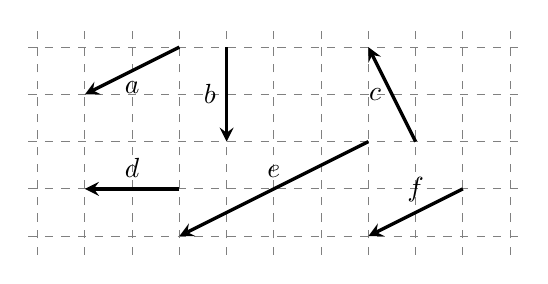
\begin{tikzpicture}[scale=0.6]
\draw [help lines,thin,dashed] (-0.2,0.6) grid (10.2,5.4);
\draw[-stealth,very thick] (3,5)--node [below] {$\vc a$} ++(-2,-1);
\draw[-stealth,very thick] (4,5)--node [left] {$\vc b$} ++(0,-2);
\draw[-stealth,very thick] (8,3)--node [left] {$\vc c$} ++(-1,2);
\draw[-stealth,very thick] (3,2)--node [above] {$\vc d$} ++(-2,0);
\draw[-stealth,very thick] (7,3)--node [above] {$\vc e$} ++(-4,-2);
\draw[-stealth,very thick] (9,2)--node [above] {$\vc f$} ++(-2,-1);
\end{tikzpicture}
\end{minipage}

\begin{enumerate}[start=3]
\itemA
\begin{enumerate}[leftmargin=1.5em,labelsep=-0.3em]
  \item A vector $\vc x$ satisfies $2(\vc a+2\vc x)-4\vc a=5(\vc x-3\vc b)$. Express $\vc x$ by $\vc a$ and $\vc b$.
 \item Vectors $\vc x$ and $\vc y$ satisfy $\vc x+\vc y=\vc a$ and $3\vc x+2\vc y=\vc b$. Express them by $\vc a$ and $\vc b$.
\end{enumerate}
\itemA Consider a triangle ABC, where $\overline{\mathrm{AB}}=1$, $\overline{\mathrm{AC}}=\sqrt5$, $\overline{\mathrm{BC}}=2$, and $\angle{\mathrm B}=90^\circ$.
Let $\vc e$ be a unit vector whose direction is the same as $\vvv{BC}$. Express $\vc e$ by $\vvv{AB}$ and $\vvv{AC}$.
 \itemA Let $\vc a=\pmat{2\\-4}$, $\vc b=\pmat{5\\ -3}$, and $\vc c=-3\vc a+2\vc b$. Find the components of $\vc c$ and calculate $|\vc c|$.
 \itemB Let $\vc a=\pmat{2\\-4}$, $\vc b=\pmat{5\\ -3}$, and $\vc p=\pmat{7\\0}$. Find $s$ and $t$ that satisfy $\vc p=s\vc a+t\vc b$.
\itemB
\begin{enumerate}[leftmargin=1.5em,labelsep=-0.3em]
\item Four points A$(2,-4)$, B$(5,-3)$, C$(2,1)$, and D are on $xy$-plane, where the quadrilateral ABCD is a parallelogram. Find the coordinate of D.
\item Two vectors $\vc a=\pmat{2\\-4}$ and $\vc b=\pmat{5+t\\-3-t}$ are parallel. What is $t$?
\end{enumerate}
\itemA
\begin{enumerate}[leftmargin=1.5em,labelsep=-0.3em]
\item Let $\vc a$ and $\vc b$ satisfy $|\vc a|=3$ and $|\vc b|=2$ and form an angle $45^\circ$. Find $\vipro a b$.
\item Let $\vc a=\pmat{2\\-4}$ and $\vc b=\pmat{5\\3}$. Find $\vipro ab$.
\end{enumerate}
\itemA
\begin{enumerate}[leftmargin=1.5em,labelsep=-0.3em]
\item Let $\vc a=\pmat{3\\7}$ and $\vc b=\pmat{-5\\-2}$. Find the angle formed by them.
\item Two vectors $\vc a=\pmat{2\\-4}$ and $\vc b=\pmat{5+x\\3+x}$ are normal to each other. Find $x$.
\end{enumerate}
\itemB Two vectors $\vc a$ and $\vc b$ satisfy $|\vc a|=3$, $|\vc b|=4$, and $|\vc a+2\vc b|=7$. Find the angle $\theta$ formed by them, assuming $0\le\theta\le\pi$.

\item[\GB{\sffamily\bfseries[12]}] \begin{enumerate}[leftmargin=1.5em,labelsep=-0.3em]
    \item Consider two points $\posvec Aa$ and $\posvec Bb$. Two points P and M are on the line AB. They are between A and B and satisfy $\overline{\mathrm{AP}}:\overline{\mathrm{PB}}=5:3$ and $\overline{\mathrm{AM}}:\overline{\mathrm{MB}}=1:1$. Describe the position vectors of P and M by using $\vc a$ and $\vc b$.
\item Consider a triangle ABC formed by three points $\posvec Aa$, $\posvec Bb$, and $\posvec Cc$. Let $\posvec Gg$ be its geometric center, and $\posvec{G'}{g'}$ be the geometric center of the triangle GBC. Describe $\vc g'$ by $\vc a$, $\vc b$, and $\vc c$.
\end{enumerate}
\item[\GC{\sffamily\bfseries[15]}] Consider a triangle ABC and let O be its circumcenter. Consider a point H satisfying $\vvv{OH}=\vvv{OA}+\vvv{OB}+\vvv{OC}$. Prove H is the orthocenter of the triangle ABC.
\end{enumerate}
\endgroup

\end{document}
